\documentclass[12pt,reqno,final]{amsart}
\usepackage[round,numbers,sort&compress]{natbib}
\usepackage{graphicx}
\usepackage{times}
\usepackage{rotating}
\usepackage{subfig}
\usepackage{Sweave}

\title[DEB fitting notes]{Fitting Dynamic Energy Budget Models:
  Parameter Covariation}

\setlength{\textwidth}{6.25in}
\setlength{\textheight}{8.75in}
\setlength{\evensidemargin}{0in}
\setlength{\oddsidemargin}{0in}
\setlength{\topmargin}{-.35in}
\setlength{\parskip}{.1in}
\setlength{\parindent}{0.0in}

\theoremstyle{plain}
\newtheorem{thm}{Theorem}
\newtheorem{corol}[thm]{Corollary}
\newtheorem{prop}[thm]{Proposition}
\newtheorem{lemma}[thm]{Lemma}
\newtheorem{defn}[thm]{Definition}
\newtheorem{hyp}[thm]{Hypothesis}
\newtheorem{example}[thm]{Example}
\newtheorem{conj}[thm]{Conjecture}
\newtheorem{algorithm}[thm]{Algorithm}
\newtheorem{remark}{Remark}
\renewcommand\thethm{\arabic{thm}}
\renewcommand{\theremark}{}

\numberwithin{equation}{part}
\renewcommand\theequation{\arabic{equation}}
\renewcommand\thesection{\arabic{section}}
\renewcommand\thesubsection{\thesection.\arabic{subsection}}
\renewcommand\thefigure{\arabic{figure}}
\renewcommand\thetable{\arabic{table}}
\renewcommand\thefootnote{\arabic{footnote}}

\begin{document}

\maketitle

I have done some initial simulation recovery experiments, and I want
to explore the results of those efforts here. Note that the
correlations among parameters for the four different parameter sets
that have been fitted can be found in
``Correlation\_among\_parameters.pdf''. In this file, I am exploring
the first parameter set.

I begin by looking at all of the estimated values for the fitted
parameters, plotted as pairwise scatterplots to look for obvious
correlations between the estimates. I focus only on those parameter
sets where the log-likelihood was within 20 units of the minimum
log-likelihood (note that subplex had not converged for \emph{any} of
these parameter sets - yikes). Points colored red are within 5
log-likelihood units of the minimum. I will focus my attention
initially on the energy allocation parameters, and show the energy
ingestion parameters and initial condition parameters next. Note that
$\nu$ is on the logarithmic scale.
\begin{figure}
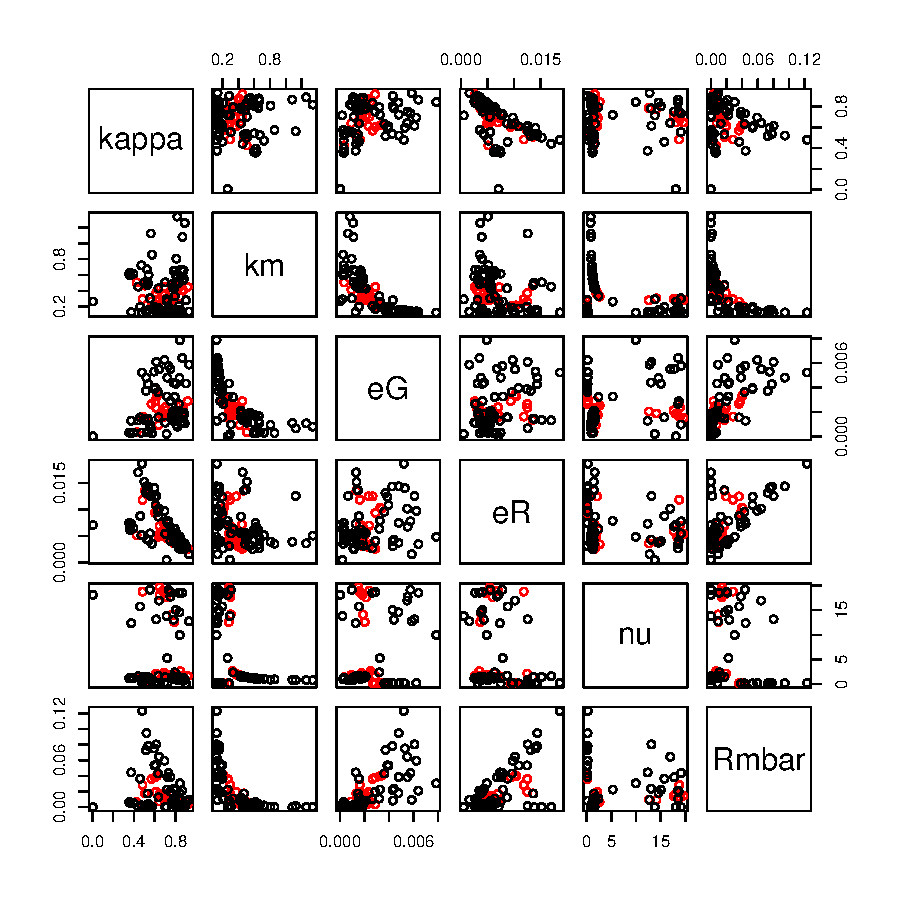
\includegraphics{Solving_the_problem_of_parameter_covariation-001}
\end{figure}

These show considerable correlation among the parameters. For example,
the estimate of the energy requirement for maturation $\bar{R_m}$ is
positively correlated with the estimate of the cost of
reproduction $\epsilon_R$, and the cost of growth $\epsilon_G$ is
negatively correlated with the somatic maintenance rate $k_m$. This
correlation is unsurprising, given that the DEB model, like
all biological models, is overparameterized. Morever, the energy
budget creates constraints that may allow parameters to trade-off
against one another, producing similar growth trajectories. It may be
that, although individual parameters cannot be well-estimated, certain
parameter combinations can be, and the model can be reparameterized in
terms of these estimable \emph{compound} parameters.

The ingestion parameters are, on the whole, badly identified. This can
be seen from the fact that most of the estimates of assimilation
efficiency $\epsilon_A$ are clustered near unity, when the truth was
0.7, and by the fact that maximum surface-area specific assimilation
rate $p_{am}$ and half-saturation constant $F_h$ have to be plotted on
the log scale.

\begin{figure}
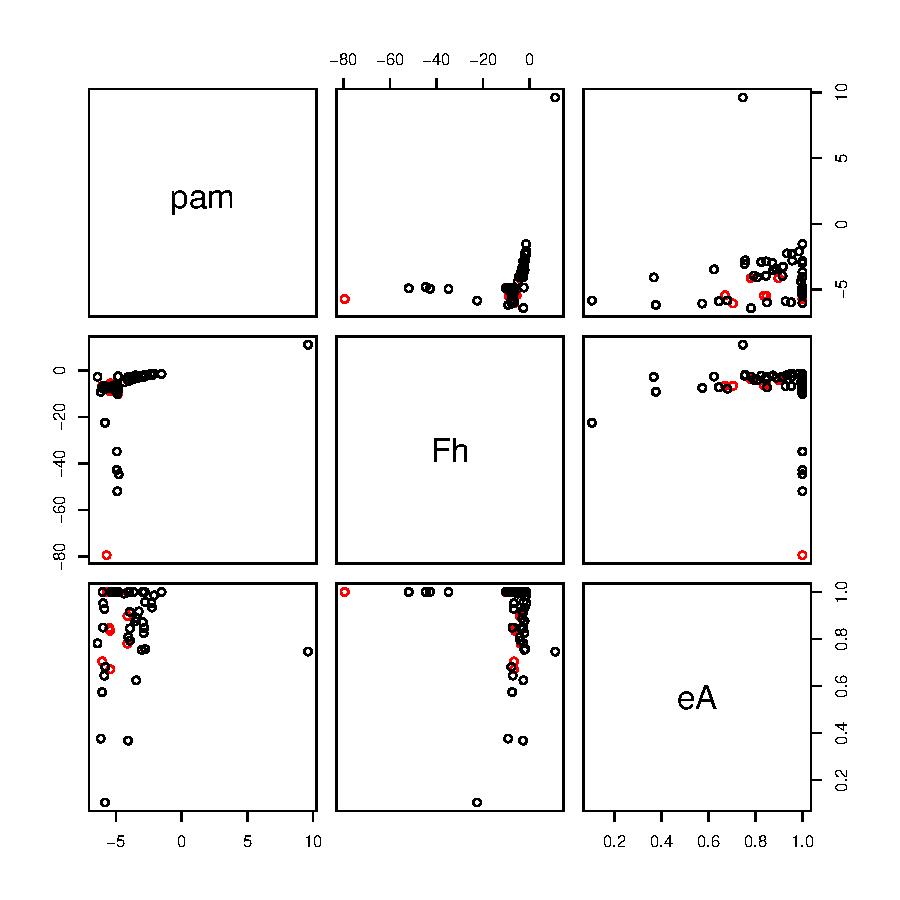
\includegraphics{Solving_the_problem_of_parameter_covariation-002}
\end{figure}

Many of the estimates of $p_{am}$ and $F_h$ are clustered
appear to cluster; unfortunately, this cluster is not actually at the
true parameter values, as can be seen in a scatterplot of just
$p_{am}$ and $F_h$, with the truth plotted in red.

\begin{figure}
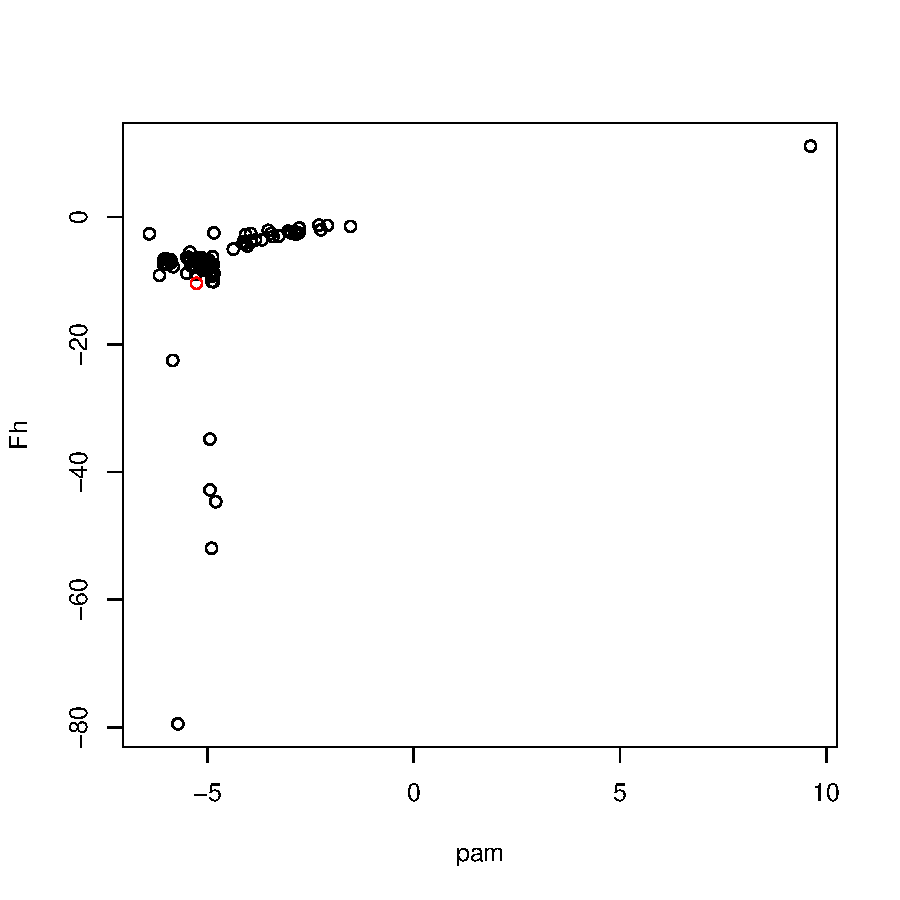
\includegraphics{Solving_the_problem_of_parameter_covariation-003}
\end{figure}

Given that the ingestion parameters seem to be difficult to estimate,
a problem that is unsurprising given that we are only considering data
at a single food level, I will focus my attention on the energy
allocation parameters only.

Let's first look at the estimates for each parameter by creating a
histogram of the ratio of the estimates to the true value - a
histogram with peak at, or near, unity inidicates that the parameter
was well-estimated. The red line indicates the truth, the blue line
indicates the mean parameter estimate, and the green line the median
estimate. This will allow us to focus our attention on only those
parameters that might need to be looked as ratios or products with
other parameters.
\begin{figure}
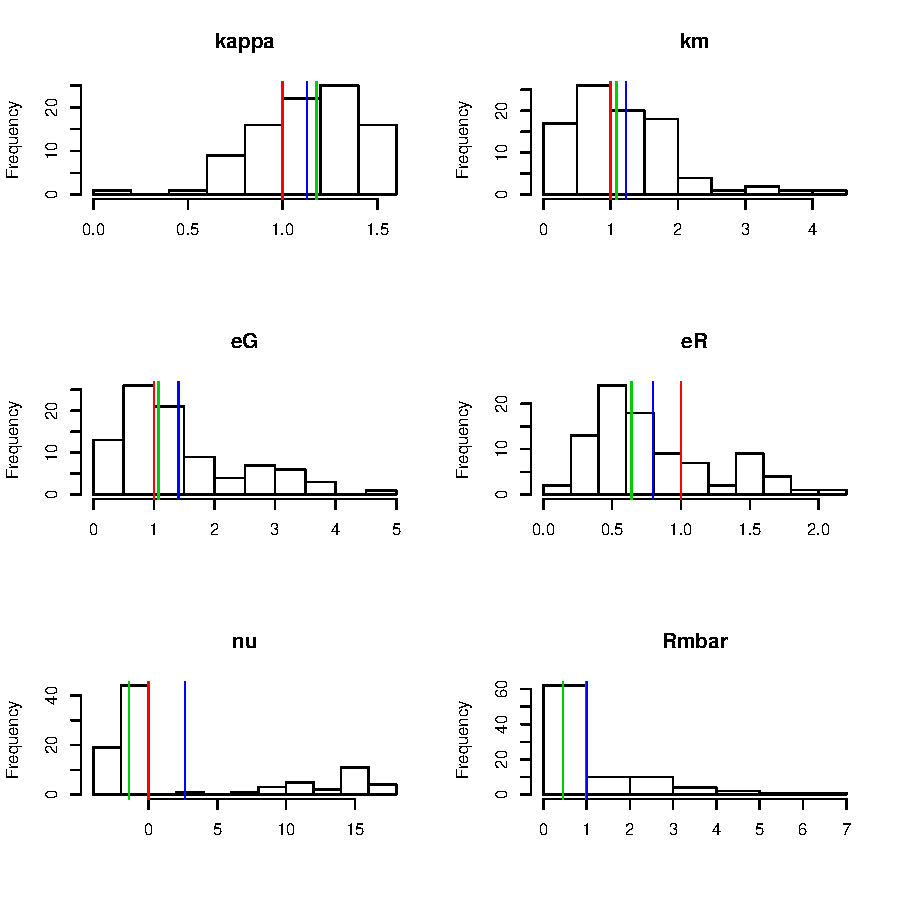
\includegraphics{Solving_the_problem_of_parameter_covariation-004}
\end{figure}

It is clear that some of the parameters are actually not very badly
estimated, in that many of the parameter sets seem to be converging to
the truth. Interestingly, the means for some of the parameters are
very close to the truth - I wonder if this is some incarnation of the
Central Limit Theorem that we can leverage? Energy conductance $\nu$ is
clearly just very difficult to estimate; it has been log-transformed
to be possible to visualize. The mean of these, surprisingly, is still
actually quite close to the truth. I had expected $\nu$ to be
difficult to estimate based on Martin et al.'s work - it works a lot
like selection strength in phylogenetic comparative hypothesis
testing. The stronger the strength of selection, the less influence
the phylogenetic history has on current traits; the larger the energy
conductance, the less influence reserve dynamics have on growth and
reproduction. As $\nu$ goes to infinity, the model becomes
reserveless.

Looking at the parameter values from all of the datasets, it is clear
that the fitting algorithm has a lot of degrees of freedom to adjust
parameters relative to one another. For example, one parameter set that had a
lower log-likelihood than the cutoff, but which is still illustrative,
fit a half-saturation constant value of $F_h=2e5$, compared to a true
value of 3e-5. It made this work by having $p_{am}=6.7e4$,
compared to a true value of 5.1e-3, and $\nu=2.4e6$, compared to a
true value of 18.1.

Another interesting example actually has an okay log-likelihood (about
10 log-likelihood units worse than the best). The estimate of
$\kappa$ was 0.96, implying almost no energy going to
reproduction. The algorithm surmounts this problem by having a very
low cost of growth and reproduction and the energy threshold for sexual maturity
happened at incredibly low amounts of energy.

All of these really brings the question of whether we can find
parameter combinations that are better identified into sharp focus. Even
better, are there parameter combinations that appear in the DEB model
that are well-estimated? For example, the mobilization rate of reserve
and the growth rate in length are
\begin{align}
  p_C &= L^3\left(\frac{\nu}{L} +
    k_m\right)\frac{E/L^3}{1+\frac{\kappa}{\epsilon_G} \frac{E}{L^3}} \\
  \frac{dL}{dt} &= \frac{\frac{\kappa}{\epsilon_G} p_C-km L^3}{3 L^2}.
\end{align}
In both $p_C$ and $dL/dt$, the parameter combination
$\kappa/\epsilon_G$ appears. Is this parameter combination well
estimated, even if $\kappa$ and $\epsilon_G$ are not? Again, showing a
histogram with the red line indicating the truth, the blue line
indicating the mean estimate, and the green line indicating the median
estimate, you can see that, indeed, the ratio is well-estimated (the
mean is skewed upward by some datasets that estimated very tiny, tiny
values of $e_G$. This is at least suggestive of the fact that the
model can profitably be reparameterized in terms of a new parameter
$\alpha = \kappa/eG$.

\begin{figure}
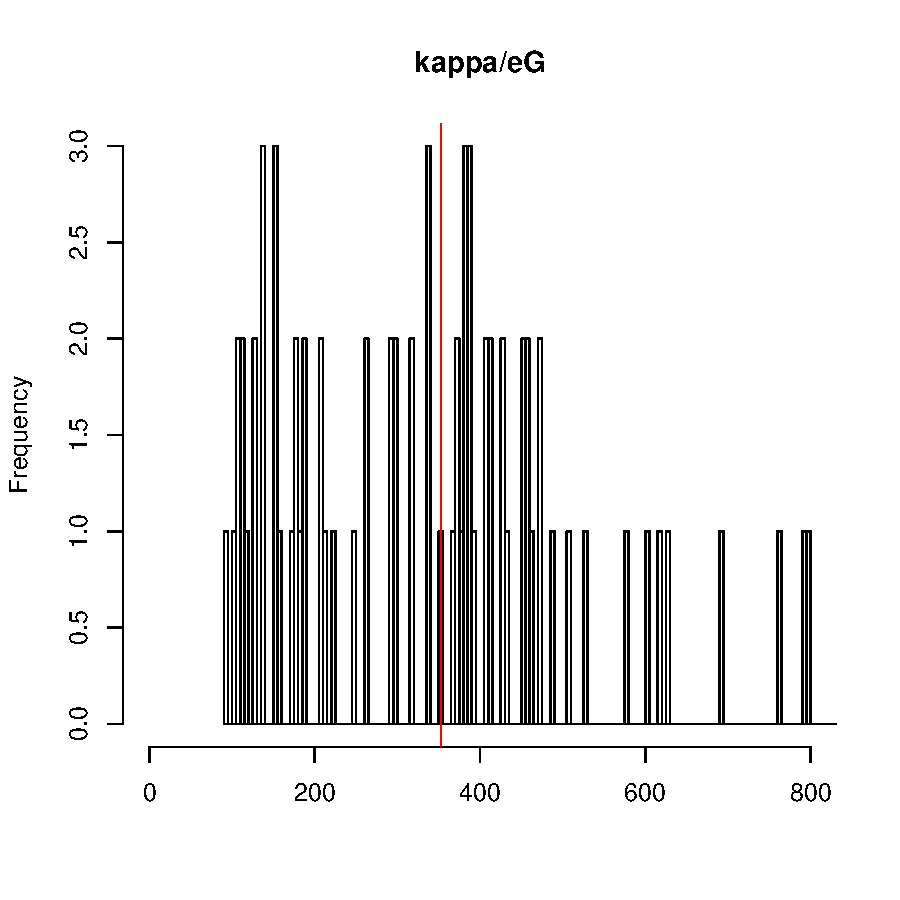
\includegraphics{Solving_the_problem_of_parameter_covariation-005}
\end{figure}

Another parameter combination that appears to be pretty well-estimated
is $k_m \epsilon_G$. Interestingly, in the derivation of the standard
DEB model, these two parameters together are the total somatic
maintenance rate $p_M$.

\begin{figure}
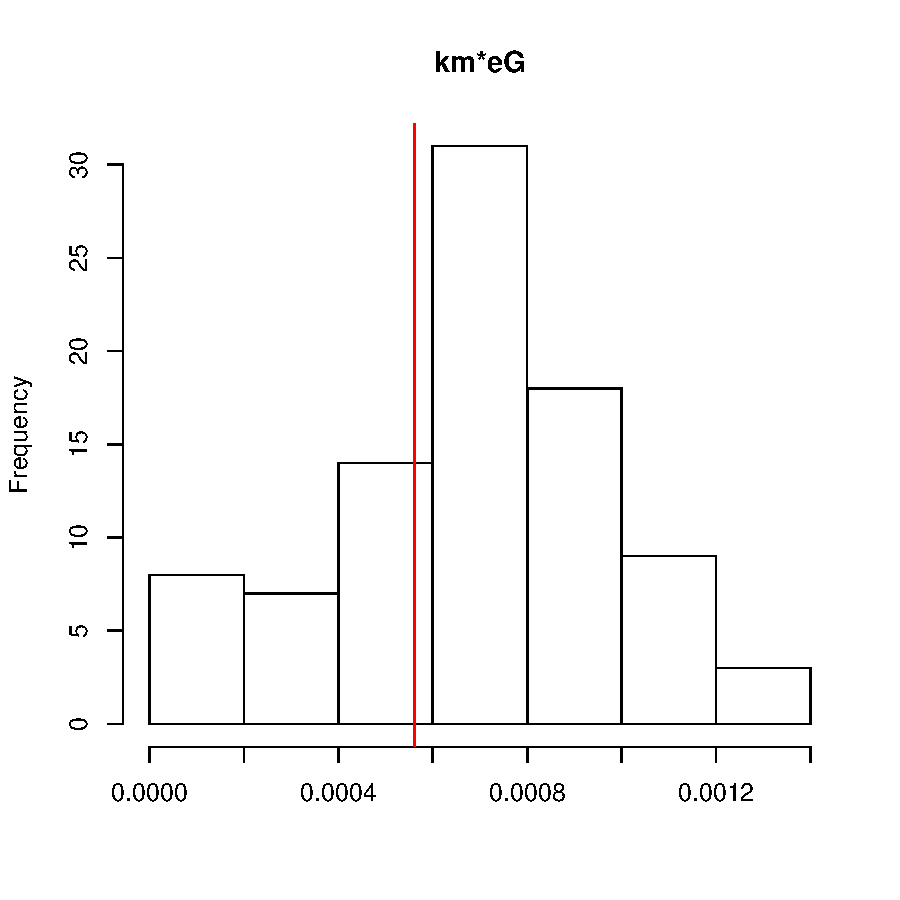
\includegraphics{Solving_the_problem_of_parameter_covariation-006}
\end{figure}

Another possibility is the ratio $\bar{R_m}$/$e_R$. Both of these
parameters deal with reproduction \emph{only}. They appear nowhere
else in the DEB dynamics. Interestingly, looking back at the pairwise
scatterplot, there almost seem to be two different lines of
correlation, with the correlation between parameters lower for
parameter sets with higher likelihood (red points). This is just a
trick of the eye, however, as you can see by overlaying histograms for
all of the data, and only the data with low likelihood score.


\begin{figure}
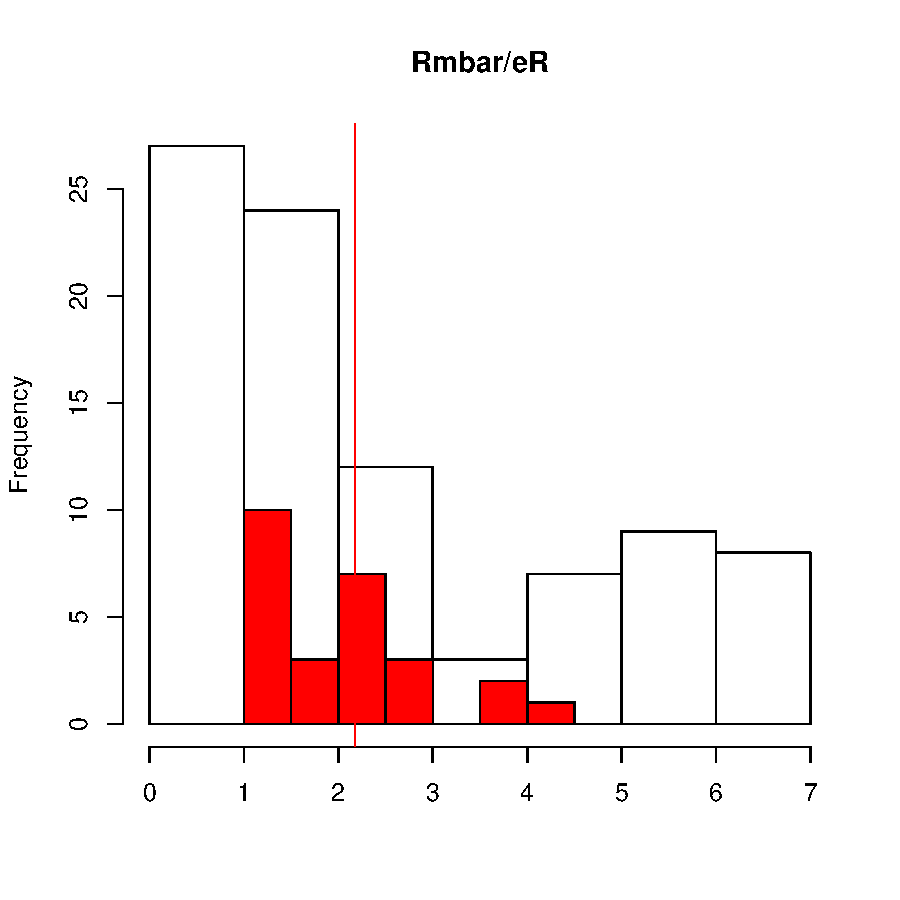
\includegraphics{Solving_the_problem_of_parameter_covariation-007}
\end{figure}

It's hard to tell initially with $\kappa/\epsilon_R$, because there
are a number of parameter sets where $\kappa$ is north of 0.96, which
forces $\epsilon_R$ to be less than 10$^{-5}$ (the most extreme is
a parameter set where $\kappa=0.99999$ and $\epsilon_R=6.5e-8$). If I
exclude these parameter sets, the histogram is much easier to
visualize, and it is clear that the estimates come very close to the truth.

\begin{figure}
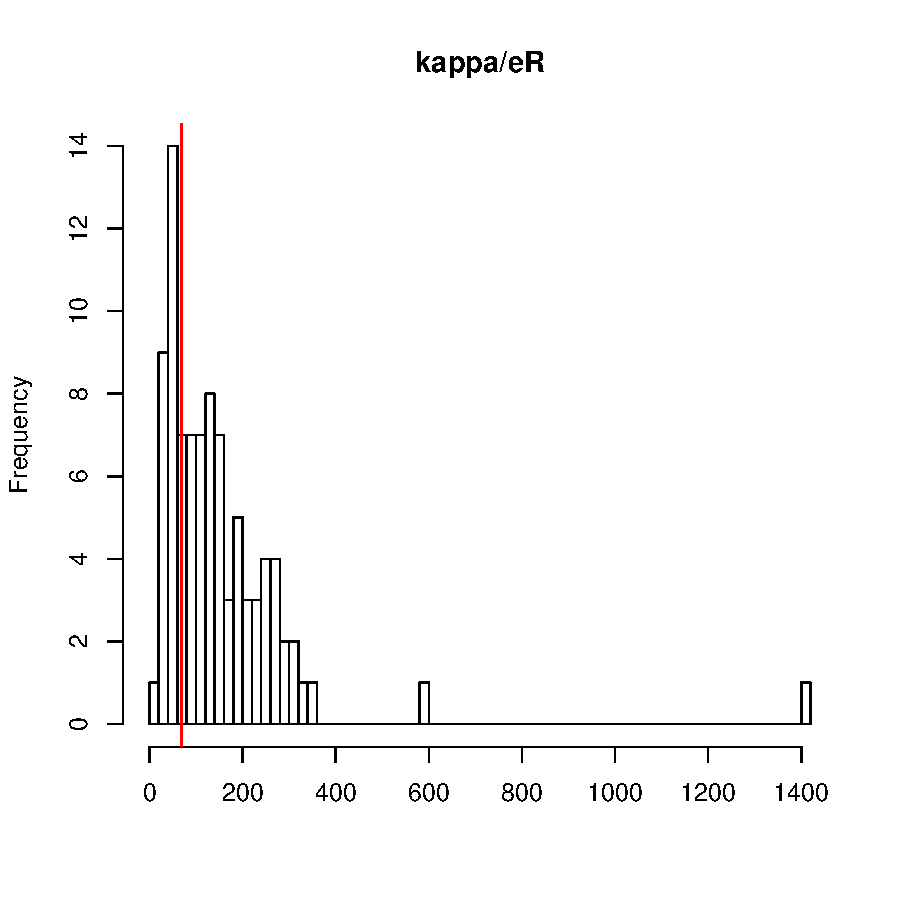
\includegraphics{Solving_the_problem_of_parameter_covariation-008}
\end{figure}

\begin{figure}
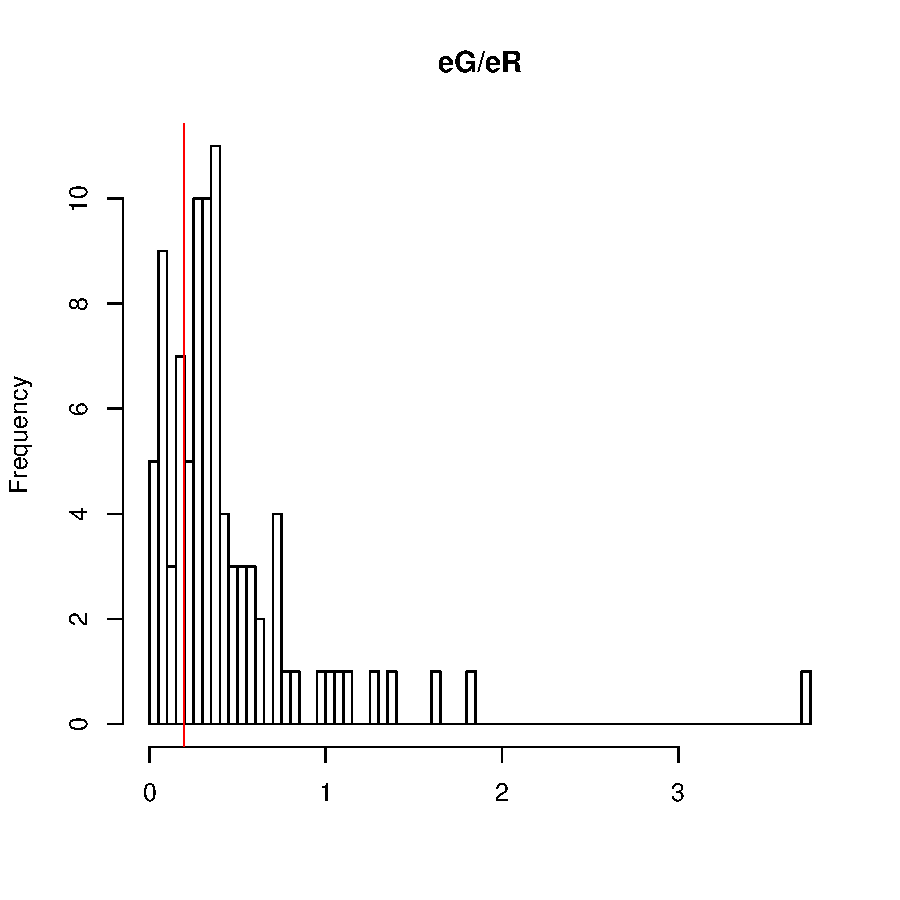
\includegraphics{Solving_the_problem_of_parameter_covariation-009}
\end{figure}


All of this is making me wonder whether it might not be better to
combine more than two parameters at the same time. In particular, I
wonder if the non-dimensionalized parameters that Bill and I were
playing around with might not be well-estimated too.

DEB theory makes use of a number of compound parameters - are any of
these well-estimated?

\begin{figure}
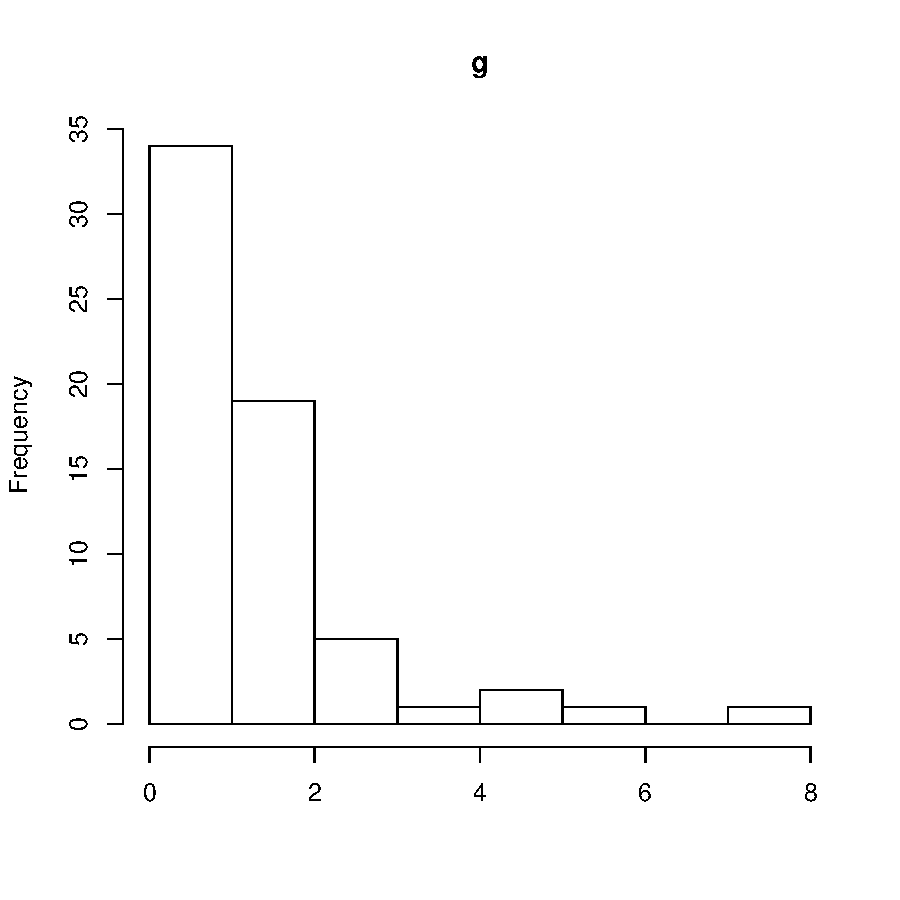
\includegraphics{Solving_the_problem_of_parameter_covariation-010}
\caption{Estimates of the DEB compound parameter $g =
  \frac{\epsilon_G \nu}{\kappa p_{am}}$, the energy investment
  ratio.}
\end{figure}

\begin{figure}
\begin{Schunk}
\begin{Sinput}
> thres <- res[-which(res[,'pam']/res[,'nu'] > 0.01),]
> hist(thres[,'pam']/thres[,'nu'],
+      main='Em', xlab='')
> abline(v=true.pars['pam']/true.pars['nu'],col=2)
\end{Sinput}
\end{Schunk}
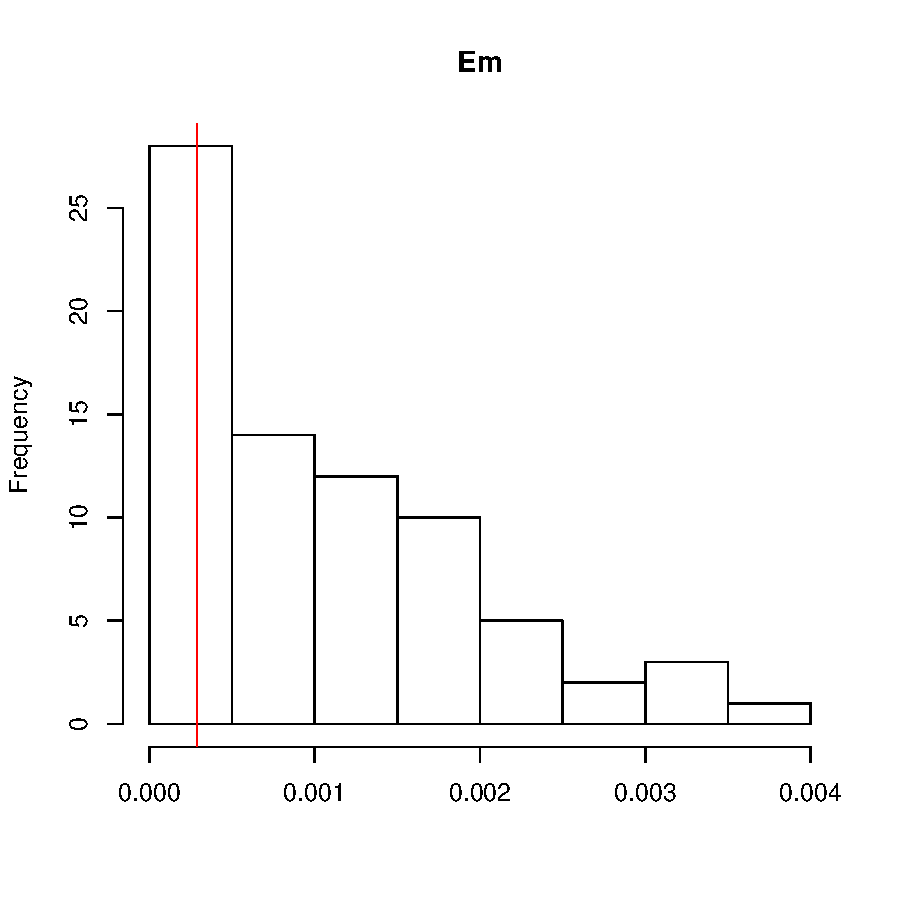
\includegraphics{Solving_the_problem_of_parameter_covariation-011}
\caption{Estimates of the DEB compound parameter $E_m = p_{am}/\nu$,
  the maximum reserve density.}
\end{figure}

\begin{figure}
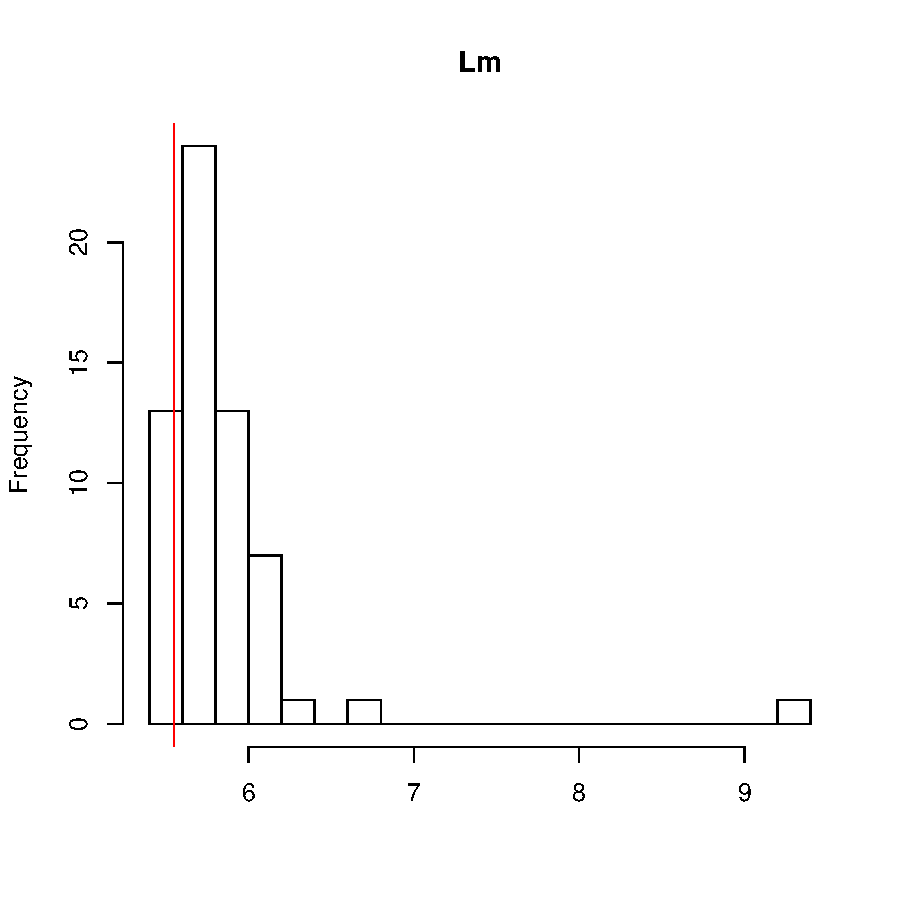
\includegraphics{Solving_the_problem_of_parameter_covariation-012}
\caption{Estimates of the DEB compound parameter $L_m = \frac{\kappa
    p_{am}}{k_m \epsilon_G}$, the maximum length.}
\end{figure}

\end{document}
